\documentclass[10pt,twocolumn,twoside]{article}

\usepackage[letterpaper,top=0.68in,bottom=0.72in,left=0.67in,right=0.67in,columnsep=0.24in]{geometry}
\usepackage{times}
\usepackage[T1]{fontenc}
\usepackage[utf8]{inputenc}
\usepackage{microtype}
\usepackage{booktabs}
\usepackage{multirow}
\usepackage{array}
\usepackage{enumitem}
\usepackage{xcolor}
\usepackage{url}
\usepackage[hidelinks]{hyperref}
\usepackage{fancyhdr}
\usepackage{tikz}
\usetikzlibrary{arrows.meta,positioning,fit,shapes.geometric}

\setlength{\parindent}{1em}
\setlength{\parskip}{0pt}
\setlength{\columnsep}{0.24in}
\setlist{nosep,leftmargin=*}
\renewcommand{\abstractname}{ABSTRACT}

\pagestyle{fancy}
\fancyhf{}
\fancyhead[LE]{Yingjie Huang}
\fancyhead[RO]{When Does an Agent-Safety Label Require the Trajectory?}
\fancyfoot[C]{\thepage}
\renewcommand{\headrulewidth}{0pt}

\newcommand{\view}[1]{\textsc{#1}}
\newcommand{\mf}{Macro-F1}
\newcommand{\fnr}{unsafe FNR}
\newcommand{\fpr}{safe FPR}

\title{\textbf{When Does an Agent-Safety Label Require the Trajectory?\\
A Partial-View and Group-Aware Audit of ATBench}}
\author{Yingjie Huang\\
University of California, Los Angeles\\
Los Angeles, CA, USA}
\date{}

\begin{document}
\maketitle

\begin{abstract}
Agent-safety evaluators are intended to identify risks that emerge across multi-step
tool use, yet a benchmark can reward a model that predicts labels from a much
smaller and easier part of the record. We audit this possibility on ATBench, a
human-reviewed benchmark containing 1,000 agent trajectories. Each record is
rendered into controlled information views: the complete trajectory, user messages,
tool schemas, agent actions, and the final answer. A class-balanced word TF--IDF
logistic classifier is evaluated with paired out-of-fold predictions under both
stratified random cross-validation and label-free task/tool-cluster-held-out
cross-validation. On the released ATBench test records, the final-answer view
reaches 0.880 group-held-out Macro-F1, compared with 0.829 for the complete
trajectory; the paired difference is +0.051 with a conditional fixed-cluster 95\%
bootstrap interval of [+0.011,+0.091]. This result establishes strong local label
signal, but does not show that trajectories are unnecessary in deployment. The
signal survives cue masking, feature-capacity controls, 12 clustering settings, and
a risk-exposed-only subset. A second public benchmark, R-Judge, also yields stronger
action-only than full-trace lexical performance, while cross-release transfer
degradation is consistent with distribution and calibration shift. The audit identifies what a
benchmark makes predictable, separates that question from real-world fault
detectability, and provides a reproducible protocol for reporting partial-view
baselines alongside trajectory-safety scores.
\end{abstract}

\section{INTRODUCTION}

\textbf{Problem statement.}
Tool-using language-model agents can expose private data, select malicious tools,
mis-handle permissions, or carry an injected instruction across several steps. A
safety judge is therefore often shown the entire execution trace. The intended
construct is trajectory-level risk awareness: the verdict should depend on the
relationship among the user's request, available tools, intermediate actions,
observations, and outcome. A high benchmark score does not by itself establish that
an evaluator used this distributed evidence. If labels correlate with a refusal in
the last message, a tool name, or a generation template, a simpler local decision
rule can receive credit for the intended reasoning task.

\textbf{State of the art.}
AgentDojo, Agent-SafetyBench, and Agent Security Bench evaluate agents in interactive
or tool-rich settings~\cite{agentdojo,agentsafetybench,asb}. R-Judge, AgentAuditor,
TraceSafe, and ATBench instead study evaluators that read completed interaction
records~\cite{rjudge,agentauditor,tracesafe,atbench}. These resources make
trajectory-level safety measurable, while recent work shows that the reliability of
the evaluator and the validity of the measurement remain open problems
~\cite{jailjudge,policyinvariance,safetycapability}. Concurrent work demonstrates
that outcome-only judges can miss process faults whose final result still appears
correct~\cite{trajectoryjudge}. That finding establishes why trajectories can
matter in deployment. It does not establish that a public benchmark requires a
model to use them.

\textbf{Motivation and research questions.}
Partial-input baselines have exposed annotation artifacts in natural-language
inference by predicting a relation label without reading both sentences
~\cite{gururangan,poliak}. We adapt the same diagnostic principle to agent traces.
The study asks:

\begin{enumerate}[label=\textbf{RQ\arabic*:}]
    \item How much ATBench label signal is recoverable from each partial view?
    \item Does that signal persist when approximate task/tool clusters are held out?
    \item How much of the final-answer result survives removal of outcome and refusal cues?
    \item Are conclusions robust to representation capacity, cluster construction,
    structural controls, risk category, and benchmark release?
\end{enumerate}

\textbf{Contributions.}
This project contributes (1) a deterministic parser and five-view information
ablation protocol for agent trajectories; (2) paired random and group-aware
out-of-fold evaluation with uncertainty estimates; (3) controls that test lexical,
length, structural, and grouping explanations; and (4) an open CPU pipeline that
rebuilds every result from pinned public data. The intended conclusion is a
measurement statement: high partial-view performance is evidence that a label is
locally predictable. It is not evidence that the omitted trajectory is causally
irrelevant or that an outcome-only monitor is safe to deploy.

\section{BACKGROUND AND RELATED WORK}

\subsection{Agent Safety and Trajectory Evaluation}
Agents expand the unit of safety analysis from a response to a sequence of actions
and environment observations. AgentDojo focuses on prompt injection in an
executable tool environment~\cite{agentdojo}; Agent-SafetyBench covers 2,000 cases
and ten failure modes~\cite{agentsafetybench}; and Agent Security Bench studies
attacks and defenses across multiple stages of agent operation~\cite{asb}. These
benchmarks primarily evaluate the behavior of the target agent.

Our object is the evaluator. R-Judge introduced risk-awareness evaluation over 569
multi-turn records~\cite{rjudge}. AgentAuditor proposed a memory-augmented judge and
ASSEBench, a larger collection spanning safety and security~\cite{agentauditor}.
TraceSafe reports that guard performance on structured traces is strongly associated
with structured-data competence, so parsing ability can confound apparent safety
reasoning~\cite{tracesafe}. ATBench contributes 1,000 human-audited trajectories,
balanced between 503 safe and 497 unsafe cases and organized by risk source, failure
mode, and real-world harm~\cite{atbench}. The release contains one official test
split. Our fitted cross-validation results are consequently a diagnostic audit, not
an official leaderboard score.

\subsection{Judge Reliability and Benchmark Validity}
JAILJUDGE treats safety judgment itself as a learned task and studies accuracy,
explanations, and multilingual generalization~\cite{jailjudge}. Policy Invariance
shows that content-preserving rubric rewrites can flip safety verdicts
~\cite{policyinvariance}. A broader validity audit shows that prevalence, metric
choice, and the target behavior can change conclusions about agent safety
~\cite{safetycapability}. These studies vary the evaluation policy or analyze
aggregate benchmark behavior. We hold the binary label fixed and vary the evidence
available to the classifier.

\subsection{Partial-Input Diagnostics}
Hypothesis-only classifiers showed that NLI labels could be predicted from one side
of an intended two-input reasoning problem~\cite{gururangan,poliak}. A successful
partial-input model provides evidence of exploitable local signal, while failure of
such a model does not prove that a dataset is artifact-free~\cite{feng}. Random
splits can further inflate apparent generalization when related instances occur on
both sides~\cite{elangovan}. We therefore reuse identical folds across views and add
a label-free cluster-held-out condition. ATBench does not publish its original
scenario-pair identifiers, so these clusters are explicitly treated as a proxy.

\subsection{Outcome-Only Versus Process-Aware Judges}
The closest concurrent work constructs 400 trajectories with known, single-point
faults. Its outcome-only judge detects 84\% of loud faults but only 45\% of silent
faults, whereas a step-rubric judge improves silent-fault recall at higher cost
~\cite{trajectoryjudge}. That experiment measures fault detection under controlled
ground truth. Our experiment measures label recoverability in an existing public
benchmark. Together, the studies expose an important distinction: a final answer
can be highly predictive inside a dataset and still be insufficient for detecting
process failures in operation.

\section{EXPERIMENTAL METHODOLOGY}

\subsection{Dataset and Leakage Controls}
We pin the official ATBench JSON file to a specific revision and SHA-256 hash. The
1,000 records contain 503 safe and 497 unsafe labels. A normalized record preserves
event order, roles, tool calls, tool results, and completion text. The annotation
fields \texttt{reason}, \texttt{risk\_source}, \texttt{failure\_mode}, and
\texttt{real\_world\_harm} are excluded from every model input. They are used only
after prediction for error slicing. Twenty-six records lack a terminal
\texttt{Complete} action; the final-answer view marks these as missing.

\begin{figure}[t]
\centering
\resizebox{\columnwidth}{!}{%
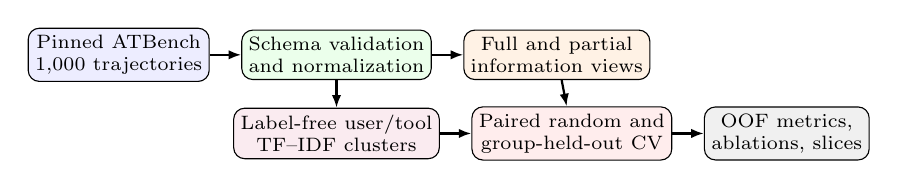
\begin{tikzpicture}[
  node distance=3.5mm and 4mm,
  box/.style={draw,rounded corners,align=center,font=\scriptsize,minimum height=6mm,inner sep=2.5pt},
  arrow/.style={-{Latex[length=1.6mm]},thick}
]
\node[box,fill=blue!7] (raw) {Pinned ATBench\\1,000 trajectories};
\node[box,fill=green!8,right=of raw] (norm) {Schema validation\\and normalization};
\node[box,fill=orange!10,right=of norm] (views) {Full and partial\\information views};
\node[box,fill=purple!8,below=of norm] (groups) {Label-free user/tool\\TF--IDF clusters};
\node[box,fill=red!7,right=of groups] (cv) {Paired random and\\group-held-out CV};
\node[box,fill=gray!12,right=of cv] (diag) {OOF metrics,\\ablations, slices};
\draw[arrow] (raw) -- (norm);
\draw[arrow] (norm) -- (views);
\draw[arrow] (norm) -- (groups);
\draw[arrow] (views) -- (cv);
\draw[arrow] (groups) -- (cv);
\draw[arrow] (cv) -- (diag);
\end{tikzpicture}
}
\caption{Audit pipeline. Labels and annotation rationales are unavailable to view construction and clustering.}
\label{fig:pipeline}
\end{figure}

\subsection{Information Views}
Each record is deterministically rendered as: \view{full}, containing tools and all
events; \view{user}, containing user messages; \view{tool}, containing available
tool schemas; \view{action}, containing tool names and arguments; and \view{final},
containing only the terminal completion text. Additional diagnostics remove the
completion from the full trace, combine user and final text, retain only trajectory
prefixes, and mask outcome/refusal cues. Every transformation is event-aware and
does not read the target label.

\begin{table}[t]
\centering
\caption{Primary ATBench view statistics.}
\label{tab:viewstats}
\scriptsize
\begin{tabular}{lrrr}
\toprule
View & Mean chars & Median chars & Missing \\
\midrule
Full trajectory & 14,630 & 7,282 & 0 \\
User only & 394 & 334 & 0 \\
Tool schema only & 3,811 & 2,779 & 0 \\
Actions only & 588 & 450 & 1 \\
Final answer only & 278 & 279 & 26 \\
\bottomrule
\end{tabular}
\end{table}

\subsection{Models and Splits}
The primary model is a class-balanced logistic regression over lowercase word
unigrams and bigrams with sublinear TF--IDF. We use the \texttt{liblinear} solver,
default $L_2$ regularization ($C=1$), and at most 1,000 iterations. It is deliberately
small: the goal is to test label accessibility, not establish the best trajectory
judge. Unless stated otherwise, the vocabulary cap is 50,000 and all preprocessing
is learned inside the training fold.

We use five-fold stratified random cross-validation and five-fold stratified grouped
cross-validation. Because the release omits scenario/template IDs, groups are
derived without labels by K-means over TF--IDF features of normalized user requests
and tool names. The main run uses 50 clusters; sensitivity experiments vary both the
cluster count and seed. All views share the same fold assignments, enabling paired
comparisons.

\subsection{Metrics and Statistical Inference}
We report Macro-F1, AUROC, balanced accuracy, unsafe false-negative rate (FNR), and
safe false-positive rate (FPR) from concatenated out-of-fold predictions. Macro-F1
prevents the nearly balanced dataset from hiding asymmetric behavior. Percentile
intervals use 500 resamples of the 50 fixed inferred clusters and fixed out-of-fold
predictions.
Paired intervals compare views on the same sampled clusters. They are conditional:
they do not include uncertainty from re-clustering, fold selection, model selection,
or exploratory analysis choices.

\section{MAIN RESULTS}

\subsection{Full and Partial Views}
Table~\ref{tab:main} reports the primary experiment. The final-answer classifier has
the highest Macro-F1 and AUROC under both split strategies. Under grouped folds it
reaches 0.880 Macro-F1 and 0.938 AUROC, compared with 0.829 and 0.903 for the full
trajectory. The paired Macro-F1 difference is +0.051 with a conditional 95\%
cluster-bootstrap interval of [+0.011,+0.091]. The corresponding random-fold
difference is +0.053 [+0.015,+0.090].

\begin{table}[t]
\centering
\caption{Out-of-fold results on all 1,000 ATBench records.}
\label{tab:main}
\scriptsize
\setlength{\tabcolsep}{3.1pt}
\begin{tabular}{llrrrr}
\toprule
Split & View & \mf{} & AUROC & FNR & FPR \\
\midrule
\multirow{5}{*}{Group}
 & Full & .829 & .903 & .179 & .163 \\
 & User & .681 & .740 & .280 & .358 \\
 & Tool & .585 & .627 & .447 & .382 \\
 & Action & .658 & .739 & .376 & .306 \\
 & \textbf{Final} & \textbf{.880} & \textbf{.938} & \textbf{.044} & .193 \\
\midrule
\multirow{5}{*}{Random}
 & Full & .821 & .895 & .189 & .169 \\
 & User & .684 & .746 & .252 & .378 \\
 & Tool & .597 & .640 & .447 & .358 \\
 & Action & .651 & .738 & .390 & .306 \\
 & \textbf{Final} & \textbf{.874} & \textbf{.937} & \textbf{.050} & .199 \\
\bottomrule
\end{tabular}
\end{table}

The error trade-off matters. Final-only dramatically reduces unsafe misses, but its
safe false-positive rate is three percentage points higher than the full model in
the grouped condition. Thus ``higher Macro-F1'' does not mean that final-only is a
strictly better operational guard.

\subsection{What the Primary Result Establishes}
The finding survives a split in which no inferred cluster appears in both training
and test folds. It therefore cannot be explained solely by exact reuse of those 50
proxy groups. It can still reflect unobserved scenario pairs, shared generation
templates, or legitimate summaries of prior behavior. The full records are also
roughly 53 times longer than final answers on average. With a fixed vocabulary cap
and document-level TF--IDF normalization, a local cue can be diluted in the full
representation. The following experiments test these alternatives rather than
interpreting Table~\ref{tab:main} as proof of leakage.

% The diagnostic and robustness sections below are populated from
% outputs/atbench-capstone after the extended experiment runner completes.

\section{DIAGNOSTIC AND ROBUSTNESS EXPERIMENTS}

\subsection{Missing Final Answers}
All 26 trajectories without a terminal completion are unsafe, making the missing
sentinel itself informative. We remove those records, preserve the original cluster
assignments for the remaining 974 examples, and rebuild the folds and model. The
group-held-out final-only result remains high: 0.871 Macro-F1, 0.934 AUROC, and
0.045 unsafe FNR. Removing records changes the evaluation population and training
sets, so the difference does not estimate the sentinel's causal contribution. It
does show that the observed result is not carried only by 26 missing values.

\subsection{Outcome Cues and Information Path}
Table~\ref{tab:informationpath} follows the information path under the primary
group folds. Static context (user plus tool schemas) reaches only 0.615 Macro-F1.
Keeping the first 25\%, 50\%, and 75\% of each record's events produces a monotonic
0.650, 0.720, and 0.754. The full trace without its completion reaches 0.766; adding
all evidence raises this to 0.829. In contrast, user plus final text reaches 0.884.
The terminal outcome is therefore the largest single local source in this lexical
representation, while the rising prefix curve also shows cumulative pre-outcome
signal.

\begin{table}[t]
\centering
\caption{Information-path ablation, group-held-out OOF.}
\label{tab:informationpath}
\scriptsize
\begin{tabular}{lrrr}
\toprule
View & Mean chars & \mf{} & FNR \\
\midrule
Static context & 4,230 & .615 & .396 \\
Prefix 25\% & 5,960 & .650 & .378 \\
Prefix 50\% & 9,355 & .720 & .310 \\
Prefix 75\% & 12,339 & .754 & .264 \\
Full without final & 14,223 & .766 & .239 \\
Full & 14,630 & .829 & .179 \\
Final only & 278 & .880 & .044 \\
User + final & 698 & \textbf{.884} & .089 \\
\bottomrule
\end{tabular}
\end{table}

The character counts in Table~\ref{tab:informationpath} are descriptive rather than
token budgets. User-plus-final has a higher FNR than final alone despite slightly
higher Macro-F1, again showing that one aggregate score does not dominate the error
trade-off.

\textbf{Cue masking.}
A transparent, post-hoc lexicon replaces refusal, authorization, policy, and
successful-outcome phrases with one neutral token. It matches 942 records and 1,941
spans, yet reduces group Macro-F1 by only 0.004, from 0.880 to 0.877. Because the
lexicon was designed after inspecting the corpus, this is exploratory. A stricter
procedure selects the largest absolute-coefficient unigram features from each
training fold only, removes them from both train and test text in that fold, and
refits the model. Removing 5, 10, 25, 50, and 100 features yields 0.875, 0.869,
0.859, 0.851, and 0.825 Macro-F1. The gradual decline indicates that the signal is
distributed across more than a short refusal/success dictionary; removing 100
fold-specific cues reduces final-only performance to approximately the unmodified
full baseline.

\begin{figure}[t]
\centering
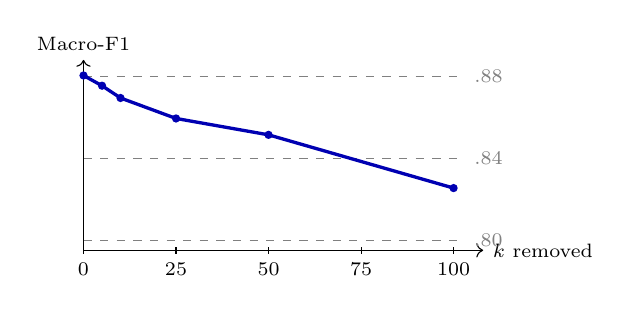
\begin{tikzpicture}[x=0.047cm,y=0.52cm,font=\scriptsize]
  \draw[->] (0,0) -- (108,0) node[right] {$k$ removed};
  \draw[->] (0,0) -- (0,4.65) node[above] {Macro-F1};
  \foreach \x in {0,25,50,75,100} {\draw (\x,0.08)--(\x,-0.08) node[below] {\x};}
  \draw[dashed,gray] (0,0.25) -- (103,0.25) node[right] {.80};
  \draw[dashed,gray] (0,2.25) -- (103,2.25) node[right] {.84};
  \draw[dashed,gray] (0,4.25) -- (103,4.25) node[right] {.88};
  \draw[very thick,blue!70!black]
    (0,4.27) -- (5,4.02) -- (10,3.72) -- (25,3.22) -- (50,2.82) -- (100,1.52);
  \foreach \x/\y in {0/4.27,5/4.02,10/3.72,25/3.22,50/2.82,100/1.52}
    \fill[blue!70!black] (\x,\y) circle (1.5pt);
\end{tikzpicture}
\caption{Leakage-controlled removal of training-fold coefficient features from final answers. The vertical scale spans approximately .80--.88 Macro-F1.}
\label{fig:cueremoval}
\end{figure}

\subsection{Feature Capacity, Structure, and Group Sensitivity}
The fixed 50,000-feature vocabulary is a plausible disadvantage for long documents.
Table~\ref{tab:robustness} confirms that representation capacity changes the gap:
with 5,000 features, full reaches 0.849 and final reaches 0.884, a difference of
0.035. Increasing the cap does not rescue full; its Macro-F1 decreases to 0.797 with
the unconstrained vocabulary, while final remains 0.880. This pattern is consistent
with sparse long-document variance or TF--IDF dilution. It rules out the narrower
claim that final's advantage exists only because full was capped at 50,000 features.

A standardized logistic model over 23 label-free numeric features---event counts,
role counts, lengths, tool-call/result balance, transitions, tool diversity, and
completion position---reaches 0.803 Macro-F1 and 0.903 AUROC. ATBench therefore has
substantial structural signal even without lexical content. This control includes
completion presence, so it is diagnostic rather than a proposed judge.

We repeat the grouping procedure for $K\in\{25,50,75,100\}$ and seeds
$\{7,21,42\}$. Across the 12 conditions, full ranges from 0.815 to 0.835 and final
from 0.870 to 0.880. The paired final-minus-full difference averages 0.050
($s=0.007$) and ranges from 0.035 to 0.061. The conclusion is stable across this
heuristic grid, although no grid can recover unpublished scenario-pair IDs.

\begin{table}[t]
\centering
\caption{Capacity and grouping robustness (group OOF Macro-F1).}
\label{tab:robustness}
\scriptsize
\begin{tabular}{lrrr}
\toprule
Control & Full & Final & $\Delta$ \\
\midrule
5k word features & .849 & .884 & +.035 \\
20k word features & .848 & .880 & +.032 \\
50k word features & .829 & .880 & +.051 \\
All word features & .797 & .880 & +.083 \\
\midrule
12 cluster settings (range) & .815--.835 & .870--.880 & .035--.061 \\
\bottomrule
\end{tabular}
\end{table}

\subsection{Taxonomy-Sliced Errors and Cross-Release Transfer}
Taxonomy labels are used only after OOF prediction. The most important asymmetry is
the \texttt{benign} risk-source slice: all 250 records are safe, and final-only flags
27.6\% of them, compared with 8.0\% for full. On the remaining 750 risk-exposed
records (253 safe, 497 unsafe), we recompute 50 label-free clusters and refit all
models. Final-only reaches 0.940 Macro-F1, 0.947 AUROC, 0.010 FNR, and 0.134 FPR;
full reaches 0.831, 0.913, 0.080, and 0.277. Thus the final-answer result does not
disappear after removing benign negatives. Instead, final text sharply separates safe and
unsafe variants once a risk-bearing scenario is present, while ordinary benign
completions are flagged more often.

\begin{table}[t]
\centering
\caption{Risk-exposed-only group CV ($n=750$).}
\label{tab:riskexposed}
\scriptsize
\begin{tabular}{lrrrr}
\toprule
View & \mf{} & AUROC & FNR & FPR \\
\midrule
Full & .831 & .913 & .080 & .277 \\
Full without final & .718 & .817 & .147 & .431 \\
User & .534 & .604 & .135 & .775 \\
Final & \textbf{.940} & .947 & .010 & .134 \\
User + final & .937 & .936 & \textbf{.006} & .150 \\
\bottomrule
\end{tabular}
\end{table}

\textbf{Cross-release transfer.}
We train on all labeled records from one official ATBench release and apply the
model and fixed 0.5 threshold to the other without target calibration. ATBench to
ATBench500 final-only retains 0.774 Macro-F1 and 0.865 AUROC, but the reverse
direction falls to 0.397 Macro-F1 and 0.607 AUROC with a 0.938 FPR. Full-transfer
Macro-F1 is approximately 0.33 in both directions. Local label signals therefore
do not imply a stable cross-release decision rule; the transfer degradation is
consistent with distribution and calibration shift.

\begin{table}[t]
\centering
\caption{Fixed-threshold cross-release transfer.}
\label{tab:transfer}
\scriptsize
\setlength{\tabcolsep}{3pt}
\begin{tabular}{llrrrr}
\toprule
Train $\rightarrow$ test & View & \mf{} & AUROC & FNR & FPR \\
\midrule
ATB $\rightarrow$ ATB500 & Full & .336 & .289 & .664 & .664 \\
 & Final & .774 & .865 & .424 & .008 \\
ATB500 $\rightarrow$ ATB & Full & .334 & .415 & .000 & .998 \\
 & Final & .397 & .607 & .000 & .938 \\
\bottomrule
\end{tabular}
\end{table}

\subsection{External Replication on R-Judge}
R-Judge has no terminal-answer marker, so we do not relabel its last action as a
final response. We pin the public repository, remove two later rows that exactly
duplicate earlier judge inputs (profile plus contents), and evaluate 569 records
(269 safe, 300 unsafe). Five-fold grouped CV keeps each of the 27 source JSON files
wholly within one fold. Full reaches 0.803
Macro-F1; all agent actions reach 0.926; and the last-action proxy reaches 0.917.
The paired last-action-minus-full difference is +0.114 with a fixed-source-group
95\% bootstrap interval of [+0.052,+0.180]. User-only reaches 0.642. This replication
shows that strong local action text is not unique to ATBench, though R-Judge's last
action is semantically broader than a final answer and the coarse source-file split
does not recover latent templates.

\begin{table}[t]
\centering
\caption{R-Judge source-file-held-out replication ($n=569$).}
\label{tab:rjudge}
\scriptsize
\begin{tabular}{lrrrr}
\toprule
View & \mf{} & AUROC & FNR & Mean chars \\
\midrule
Full & .803 & .902 & .080 & 1,782 \\
User only & .642 & .701 & .223 & 140 \\
Action only & \textbf{.926} & .975 & .043 & 483 \\
Last action & .917 & .969 & .053 & 343 \\
\bottomrule
\end{tabular}
\end{table}

\section{DISCUSSION}

\textbf{Benchmark interpretation.}
The primary result says that a low-capacity lexical model can recover a large amount
of ATBench's binary-label signal from final answers. It does not say that the label
is wrong. A refusal or confirmation can be a faithful summary of whether the agent
executed an unsafe request. The concern is construct coverage: if a reported score
is intended to demonstrate multi-step reasoning, a strong final-only baseline means
that the score alone cannot establish that the evaluator used intermediate evidence.

\textbf{Practical interpretation.}
A cheap final-answer classifier may be useful for triage, but the asymmetric errors
in Table~\ref{tab:main} rule out replacing trace review on the basis of this audit.
Controlled fault injection shows that correct-looking outcomes can hide unsafe
processes~\cite{trajectoryjudge}. A deployment policy should therefore evaluate
coverage and escalation cost on process-fault data rather than select the shortest
view solely by in-benchmark F1.

\textbf{Recommendations for benchmark reporting.}
Trajectory-safety datasets should publish scenario and pair identifiers, keep whole
families in the same split, report majority/structure/partial-view baselines, and
separate outcome-visible failures from failures requiring cross-step evidence.
Judge cards should state the exact policy, input representation, truncation, class
prevalence, and FNR/FPR trade-off. These additions do not replace full evaluator
benchmarks; they make the evidence behind a benchmark score easier to audit.

\section{THREATS TO VALIDITY}

\textbf{Single benchmark and exploratory reuse.}
ATBench provides only an official test release. We inspect it, derive clusters, fit
models, and choose diagnostics on the same 1,000 records. Cross-validation prevents
direct train/test reuse within a run but does not create an untouched confirmatory
dataset. Extended cross-release results reduce but do not eliminate this limitation.

\textbf{Proxy grouping.}
The original scenario skeleton and pair IDs are not public. User/tool clusters are
transductive lexical proxies and may split true variants or merge unrelated tasks.
Cluster-count and seed sensitivity quantifies only the instability of this heuristic,
not recovery of the unavailable ground truth.

\textbf{Model and representation.}
TF--IDF logistic regression measures accessible lexical signal, not the capability
of an LLM judge. Full trajectories are much longer than partial views, and feature
truncation or normalization may disadvantage them. Capacity and information-path
controls address known mechanisms, but no finite set of baselines identifies the
causal source of performance.

\textbf{Conditional uncertainty.}
Bootstrap intervals condition on fitted OOF predictions and fixed clusters. They do
not cover researcher degrees of freedom, re-clustering, refitting, or model-family
selection. Taxonomy slices are descriptive and can be small; they are not treated as
independent confirmatory hypothesis tests.

\textbf{External validity.}
ATBench trajectories are generated and human-audited benchmark artifacts, not logs
sampled from a deployed agent population. Predictability within this release cannot
establish calibration, robustness to adaptive agents, or safety under distribution
shift.

\section{CONCLUSION}

\textbf{Future work.}
The strongest next step is a frozen evaluation on an external trajectory benchmark
with published task-family IDs, followed by a compact trajectory-native judge under
the same views. A manually verified paired subset could intervene on final-answer
wording while holding the action trace fixed, yielding stronger causal evidence than
observational masking.

\textbf{Final thoughts.}
Existing research establishes that full trajectories can contain safety-critical
evidence. This capstone asks the complementary measurement question: does a benchmark
score require an evaluator to use that evidence? On exploratory ATBench
cross-validation, final answers alone expose a strong binary-label signal. Treating
that result as a prompt for stricter controls---rather than as proof that trajectories
are unnecessary---produces a more informative audit and a practical reporting
standard for future agent-safety benchmarks.

\begin{thebibliography}{99}
\small

\bibitem{atbench}
Y. Li et al., ``ATBench: A Diverse and Realistic Trajectory Benchmark for Long-Horizon Agent Safety,'' arXiv:2604.02022, 2026.

\bibitem{rjudge}
T. Yuan et al., ``R-Judge: Benchmarking Safety Risk Awareness for LLM Agents,'' in \textit{Findings of EMNLP}, 2024.

\bibitem{agentauditor}
H. Luo et al., ``AgentAuditor: Human-Level Safety and Security Evaluation for LLM Agents,'' in \textit{NeurIPS}, 2025.

\bibitem{tracesafe}
Y.-S. Chen, S.-Y. Huang, C.-L. Yang, and Y.-N. Chen, ``TraceSafe: A Systematic Assessment of LLM Guardrails on Multi-Step Tool-Calling Trajectories,'' arXiv:2604.07223, 2026.

\bibitem{agentdojo}
E. Debenedetti et al., ``AgentDojo: A Dynamic Environment to Evaluate Prompt Injection Attacks and Defenses for LLM Agents,'' arXiv:2406.13352, 2024.

\bibitem{agentsafetybench}
Z. Zhang et al., ``Agent-SafetyBench: Evaluating the Safety of LLM Agents,'' arXiv:2412.14470, 2024.

\bibitem{asb}
H. Zhang et al., ``Agent Security Bench (ASB): Formalizing and Benchmarking Attacks and Defenses in LLM-Based Agents,'' arXiv:2410.02644, 2024.

\bibitem{jailjudge}
F. Liu et al., ``JAILJUDGE: A Comprehensive Jailbreak Judge Benchmark with Multi-Agent Enhanced Explanation Evaluation Framework,'' arXiv:2410.12855, 2024.

\bibitem{policyinvariance}
S. Weng, Y. Feng, and X. Xie, ``Beyond Accuracy: Policy Invariance as a Reliability Test for LLM Safety Judges,'' arXiv:2605.06161, 2026.

\bibitem{safetycapability}
Y. Wang, X. Han, D. Shang, Y. Tang, and B. Liu, ``Safety, or Just Capability? A Validity Audit of Agent-Safety Benchmarks,'' arXiv:2607.28685, 2026.

\bibitem{trajectoryjudge}
H. Mohammadi, ``trajectory-judge: What Outcome-Only LLM Judges Miss on Agent Trajectories,'' arXiv:2609.00038, 2026.

\bibitem{gururangan}
S. Gururangan et al., ``Annotation Artifacts in Natural Language Inference Data,'' in \textit{NAACL-HLT}, pp. 107--112, 2018.

\bibitem{poliak}
A. Poliak, J. Naradowsky, A. Haldar, R. Rudinger, and B. Van Durme, ``Hypothesis Only Baselines in Natural Language Inference,'' in \textit{*SEM}, pp. 180--191, 2018.

\bibitem{feng}
S. Feng, E. Wallace, and J. Boyd-Graber, ``Misleading Failures of Partial-Input Baselines,'' in \textit{ACL}, pp. 5533--5538, 2019.

\bibitem{elangovan}
A. Elangovan, J. He, and K. Verspoor, ``Memorization vs. Generalization: Quantifying Data Leakage in NLP Performance Evaluation,'' in \textit{EACL}, pp. 1325--1335, 2021.

\bibitem{shortcut}
R. Geirhos et al., ``Shortcut Learning in Deep Neural Networks,'' \textit{Nature Machine Intelligence}, vol. 2, pp. 665--673, 2020.

\end{thebibliography}
\end{document}
